\documentclass[tikz,border=10pt]{standalone}
\usepackage{amsmath,amssymb}
\usepackage{tikz}
\usetikzlibrary{arrows.meta,calc,positioning}

\definecolor{navy}{HTML}{1B365D}
\definecolor{steelblue}{HTML}{2471A3}
\definecolor{teal}{HTML}{0E6251}
\definecolor{amber}{HTML}{D35400}
\definecolor{crimson}{HTML}{C0392B}
\definecolor{slate}{HTML}{566573}

\begin{document}
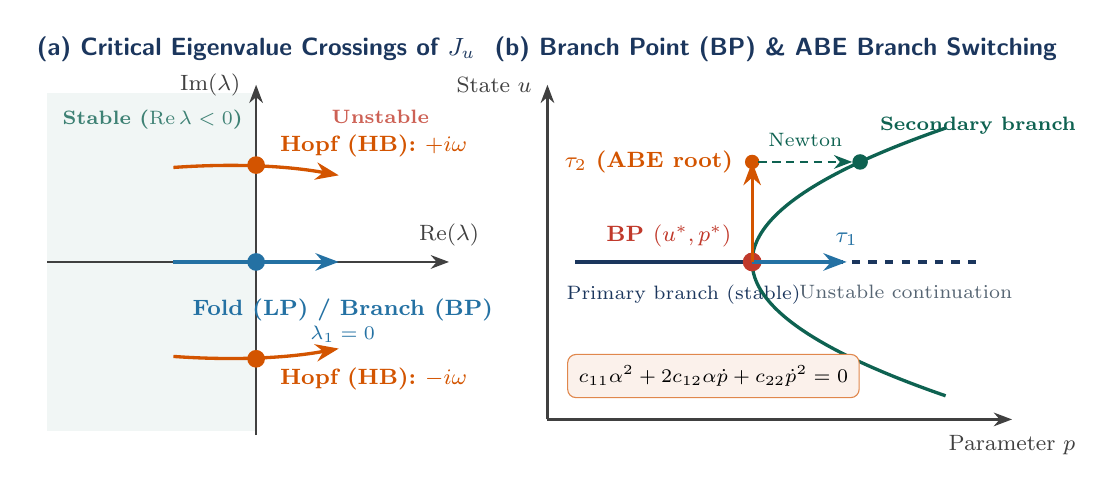
\begin{tikzpicture}[
    >=Stealth,
    font=\sffamily\small,
]

% ========================
% LEFT PANEL: Complex Eigenvalue Plane (LP/BP vs Hopf)
% ========================
\begin{scope}[shift={(0,0)}]
    \node[font=\sffamily\bfseries\small, navy] at (2.4, 5.15)
        {(a) Critical Eigenvalue Crossings of $J_u$};

    % Stable half-plane shading
    \fill[teal!6] (-0.25, 0.3) rectangle (2.4, 4.6);
    \node[teal!80, font=\scriptsize\bfseries, anchor=north west] at (-0.18, 4.50) {Stable ($\operatorname{Re}\lambda < 0$)};
    \node[crimson!80, font=\scriptsize\bfseries, anchor=north east] at (4.72, 4.50) {Unstable};

    % Axes
    \draw[->, thick, black!75] (-0.25, 2.45) -- (4.85, 2.45) node[above=2pt, font=\footnotesize] {$\operatorname{Re}(\lambda)$};
    \draw[->, thick, black!75] (2.4, 0.25) -- (2.4, 4.70) node[left=2pt, font=\footnotesize] {$\operatorname{Im}(\lambda)$};

    % LP / BP crossing along real axis
    \draw[->, very thick, steelblue] (1.35, 2.45) -- (3.45, 2.45);
    \fill[steelblue] (2.4, 2.45) circle (3.2pt);
    \node[steelblue, font=\footnotesize\bfseries, align=center, below=8pt] at (3.50, 2.38)
        {Fold (LP) / Branch (BP)\\[-1pt]\normalfont\scriptsize $\lambda_1 = 0$};

    % Hopf complex conjugate crossing
    \draw[->, very thick, amber] (1.35, 3.65) .. controls (2.05, 3.70) and (2.75, 3.68) .. (3.45, 3.55);
    \draw[->, very thick, amber] (1.35, 1.25) .. controls (2.05, 1.20) and (2.75, 1.22) .. (3.45, 1.35);
    \fill[amber] (2.4, 3.68) circle (3.2pt);
    \fill[amber] (2.4, 1.22) circle (3.2pt);
    \node[amber, font=\footnotesize\bfseries, anchor=west] at (2.58, 3.92) {Hopf (HB): $+i\omega$};
    \node[amber, font=\footnotesize\bfseries, anchor=west] at (2.58, 0.96) {Hopf (HB): $-i\omega$};
\end{scope}

% ========================
% RIGHT PANEL: Branch Point & ABE Branch Switching
% ========================
\begin{scope}[shift={(6.1, 0)}]
    \node[font=\sffamily\bfseries\small, navy] at (2.9, 5.15)
        {(b) Branch Point (BP) \& ABE Branch Switching};

    % Axes
    \draw[->, thick, black!75] (0.0, 0.45) -- (5.9, 0.45) node[below=2pt, font=\footnotesize] {Parameter $p$};
    \draw[->, thick, black!75] (0.0, 0.45) -- (0.0, 4.70) node[left=2pt, font=\footnotesize] {State $u$};

    % Primary branch (horizontal trivial branch u = 2.45)
    \draw[very thick, navy] (0.35, 2.45) -- (2.60, 2.45);
    \draw[very thick, navy, dashed] (2.60, 2.45) -- (5.55, 2.45);
    \node[navy, font=\scriptsize, below=4pt, anchor=north west] at (0.12, 2.42) {Primary branch (stable)};
    \node[slate, font=\scriptsize, below=4pt] at (4.55, 2.42) {Unstable continuation};

    % Secondary pitchfork branch: p = 2.60 + 0.65*(u - 2.45)^2
    \draw[very thick, teal, domain=0.75:4.15, samples=80, smooth]
        plot ({2.60 + 0.85*(\x - 2.45)*(\x - 2.45)}, {\x});
    \node[teal, font=\scriptsize\bfseries, anchor=west] at (4.10, 4.18) {Secondary branch};

    % BP point
    \coordinate (bp) at (2.60, 2.45);
    \fill[crimson] (bp) circle (3.4pt);
    \node[crimson, font=\footnotesize\bfseries, above left=2pt and 4pt] at (bp) {BP $(u^*, p^*)$};

    % Primary tangent tau_1
    \draw[->, very thick, steelblue] (bp) -- (3.80, 2.45)
        node[above=2pt, font=\footnotesize\bfseries, steelblue] {$\tau_1$};

    % Secondary tangent tau_2 (vertical at pitchfork!)
    \draw[->, very thick, amber] (bp) -- (2.60, 3.72)
        node[left=3pt, font=\footnotesize\bfseries, amber] {$\tau_2$ (ABE root)};

    % Predicted jump u_init = u* + ds * tau_2 and Newton convergence to secondary branch
    \coordinate (uinit) at (2.60, 3.72);
    \coordinate (uconv) at ({2.60 + 0.85*(1.27)*(1.27)}, 3.72);
    \fill[amber] (uinit) circle (2.6pt);
    \draw[->, thick, teal, densely dashed] ($(uinit) + (0.08, 0)$) -- ($(uconv) + (-0.10, 0)$)
        node[midway, above=2pt, font=\scriptsize, teal] {Newton};
    \fill[teal] (uconv) circle (2.8pt);

    % ABE box
    \node[draw=amber!70, fill=amber!8, rounded corners=3pt, font=\scriptsize, anchor=south west, inner sep=4pt]
        at (0.25, 0.72) {$c_{11}\alpha^2 + 2c_{12}\alpha\dot{p} + c_{22}\dot{p}^2 = 0$};
\end{scope}

\end{tikzpicture}
\end{document}
